%!TEX program = xelatex
\documentclass[letterpaper]{article}

\usepackage{aaai16}
\usepackage{times}
\usepackage{helvet}
\usepackage{courier}

\setlength{\pdfpagewidth}{8.5in}
\setlength{\pdfpageheight}{11in}

\usepackage{rotating}
\usepackage{color}
\usepackage{epsfig,subcaption,multicol,multirow}
\usepackage{epstopdf}
\usepackage{amsmath,algorithm}
\usepackage[noend]{algpseudocode}
\usepackage{textcomp}
\usepackage{graphicx}
\usepackage{url}
\usepackage{lingmacros,framed}
\usepackage[T1]{fontenc}
\newcommand{\KZ}[1]{\textcolor{blue}{Kenny: #1}}
\newcommand{\ZY}[1]{\textcolor{red}{J: #1}}
\newcommand{\tabref}[1]{Table \ref{#1}}
\newcommand{\figref}[1]{Figure \ref{#1}}
\newcommand{\secref}[1]{Section \ref{#1}}
\newcommand{\eqnref}[1]{Equation (\ref{#1})}
\newcommand{\cut}[1]{}
\newtheorem{example}{Example}

\DeclareMathOperator*{\argmax}{arg\,max}
\DeclareMathOperator*{\argmin}{arg\,min}

\pdfinfo{
/Title (Commonsense Causal Reasoning between Short Texts)
/Author (Zhiyi Luo, YuChen Sha, Kenny Q. Zhu, Seung-won Hwang, Zhongyuan Wang)}

\setcounter{secnumdepth}{2}

\begin{document}
\title{Commonsense Causal Reasoning between Short Texts}

\author{
Zhiyi Luo{\small $~^{1}$} \and Yuchen Sha{\small $~^{2}$} \and Kenny Q. Zhu{\small $~^{3}$}\\
Shanghai Jiao Tong University, Shanghai, China\\
\{{\small $^{1}$}jessherlock,{\small $^{2}$}sycbelief\}@sjtu.edu.cn,{\small $^{3}$}kzhu@cs.sjtu.edu.cn (contact author)\\
\AND
Seung-won Hwang\\
Yonsei University, Seoul, Republic of Korea\\
seungwonh@yonsei.ac.kr\\
\And
Zhongyuan Wang\\
Microsoft Research Asia, Beijing, China\\
zhy.wang@microsoft.com
}
\maketitle
\begin{abstract}
Commonsense causal reasoning is the process of capturing and understanding
the causal dependencies amongst events and actions.
Such events and actions can be expressed in terms, phrases or
sentences in natural language text.
Therefore, one possible way of obtaining causal knowledge is by extracting
causal relations between terms or phrases from a large text corpus.
However, causal relations in text are sparse, ambiguous, and sometimes implicit,
and thus difficult to obtain.
This paper attacks the problem of commonsense causality reasoning between short
texts (phrases and sentences) using a data driven approach.
We propose a framework that automatically harvests a network of
causal-effect terms from a large web corpus.
Backed by this network, we propose a novel and effective metric to properly
model the causality strength between terms. We show these signals
can be aggregated for causality reasonings between
short texts, including sentences and phrases.
In particular, our approach outperforms all previously
reported results in the standard SEMEVAL COPA task by substantial margins.
\end{abstract}

% \input{intro}
\section{Introduction}
\label{sec:intro}

Commonsense causal reasoning, a central challenge in artificial intelligence,
has been actively studied by both linguists and computer scientists.
It aims at understanding the general causal dependency
between common events or actions.
Such understanding essentially amounts to measuring the {\em plausibility} of
one event statistically leading to another.

In this paper, we focus on commonsense causal reasoning between short texts,
which is crucial to many natural language processing applications,
such as text understanding, question answering, etc.
To further illustrate commonsense causal reasoning problem,
we present a question from Choice of Plausible Alternatives (COPA)
evaluation~\cite{roemmele2011choice}
which consists of one thousand multiple-choice questions requiring
commonsense causal reasoning to answer correctly.
Specifically, each question is composed of a premise and two
alternatives, where the task is to select the more plausible
alternative as a cause (or effect) of the premise.

\begin{example}
\label{ex:copa}
%\noindent
\begin{itemize}
\item[] Premise: \emph{I knocked on my neighbor's door.} What
happened as an effect?
\item[] Alternative 1: \emph{My neighbor invited me in.}
\item[] Alternative 2: \emph{My neighbor left her house.}
\end{itemize}
\end{example}

This example shows that a key challenge is
harvesting causality knowledge that the action of
{\em knocking} is more likely to cause that of {\em invitation}
than that of {\em leaving}.

Existing work on harvesting causality knowledge has been conducted in
two directions.
First direction, pursuing high {\em precision} of
causality knowledge, usually requires expensive manual efforts.
For example, ConceptNet~\cite{HavasiSALAM10} leverages human efforts
to encode causal events as common sense knowledge.
Khoo et al.~\shortcite{khoo2000extracting} hand-crafted
lexical syntactic patterns from the dependency tree to recognize
causal knowledge.  Rink et al.~\shortcite{rink2010learning}
automatically generated such patterns encoded with
lexical, syntactic and semantic information to extract
causality knowledge, but the approach requires initial training data,
which determines the quality and quantity of the generated patterns.
Such iterative approach also tends to bring in ill-formed patterns
and unreliable results.
Other approaches reported in~\cite{gordon2012copa} build on deeper
lexical syntactic analysis of sentences,
to identify knocking and inviting in our example as
\emph{events}, and determine whether causality between two events hold.
However, knowledge acquired by these approaches,
based on human and in-depth analysis, inherently lack coverage.

Second direction, harvesting causality from large
text corpus with a data-driven approach, seeks to overcome
the limitation in breadth of the first direction.
The best known approach~\cite{gordon2011commonsense} here,
outperforming the approaches in the first direction~\cite{gordon2012copa},
leverages personal stories as a source of information about causality and uses
Pointwise Mutual Information (PMI) statistics \cite{church1990word}
between words in the premise and alternative, to identify the pairs with
high correlation. More specifically, under this framework,
words $A$ and $B$ are considered causal, if $A$ is frequently co-located
with and succeeded by $B$ in text.
In our example, while we expect the words \emph{knock} and \emph{invite}
to co-occur frequently in narrative text, which indicates a potential causality;
the words \emph{door} and \emph{house} are also observed frequently together.
Misidentifying both as causality may incorrectly give the second
alternative as the result.
Thus implicit causality from lexical co-occurrence alone is noisy.
Therefore, current data-driven approaches may address the coverage
limitation of causality acquisition, but suffer from low precision in return.

In contrast, our goal is to pursue both coverage and precision
in modeling causality. Combining in-depth lexical syntactic analysis with
personal stories is not an option because given the limited availability
of such data,
the amount of extractable precise causal knowledge would be much smaller.
To pursue coverage, we propose a data-driven approach of harvesting
a comprehensive \emph{term-based causality network} from a large web corpus.
Such network would encode tens of thousands of unique terms,
and tens of millions of causality evidences, much larger scale than other
existing causal knowledge bases (more comparisons in \secref{sec:causalnet}).

To pursue precision, we leverage explicit causal indicators
(e.g., cause, because), to prune substantial non-causal co-occurrences and
introduce separate cause and effect roles to every term in our
causality knowledge.

With the differentiated cause and effect roles of causalities encoded in text,
our causality network carries more reasonable and
directional {\em causal co-occurrences}, e.g., from the corpus,
$knock$ causes $invite$ $m$ times, while $invite$ causes
$knock$ $n$ times. Furthermore, we distinguish sufficiency causality (i.e.,
$A$ is the sufficient condition to cause $B$) from necessity causality
(i.e., $A$ is the necessary cause of $B$).
These refined representations of terms and their causal relations
give rise to new ways of computing causal strength between
terms and between texts,
thus yields better results in commonsense causal reasoning.

In sum, this paper makes the following contributions:
\begin{itemize}
\item We harvest a term-based causality co-occurrences network from large
web text by leveraging causal cues (see \secref{sec:network});
\item We develop a new statistical metric that captures causal strength
between any two pieces of short texts (see \secref{sec:causalstrength}
and \secref{sec:reasoning});

\item Our proposed framework achieves state-of-the-art accuracy of $70.2\%$
on the difficult COPA task, outperforming all existing methods by subtantial margins.
Further evaluation on causality detection between phrases also
demonstrate the advantage of the proposed framework (see \secref{sec:eval}).
\end{itemize}

% \input{approach}
\section{Approach}
\label{sec:approach}

To reason about causality between short texts,
our framework includes i) a network of causal relation weighted with
causality co-occurrences between terms that is extracted from
a large web corpus; ii) a novel metric to compute causal strength
 between any two terms based on this network; iii)
a simple algorithm for aggregating the causality between terms to
compute the overall score for causality reasoning between short texts,
including phrases and sentences.
Next, we describe these components.

\subsection{Causality Network}
\label{sec:network}
s
Causality is expressed by natural language texts and can be identified by
linguistic patterns known as {\em causal cues}~\cite{ChangC04}.
Consider the following sentences:
\enumsentence{
The [{\em {storm}}]\textsubscript{{\sc cause}} [{\bf caused}]\textsubscript{{\sc pattern}} a tremendous amount of [{\em damage}]\textsubscript{{\sc effect}} on the landing beaches.
}

\enumsentence{The team prepared GIS precipitation and contour maps of the area
identifying the [{\em flooding}]\textsubscript{{\sc effect}} and landslides [{\bf caused by}]\textsubscript{{\sc pattern}} the [{\em rainfall}]\textsubscript{{\sc cause}}.
}

\enumsentence{However Susanoo was in [{\em sorrow}]\textsubscript{{\sc effect}} after the [{\em loss}]\textsubscript{{\sc cause}} of his mother and he was raging in his kingdom. 
}
In sentence (1),
`storm' is the cause of `damage', and `damage' is the effect of `storm'.
We exploit {\em causal cues} (causal patterns) shown in \tabref{tab:cue},
to identify cause and effect roles for our causality knowledge.
For example, \textit{``A cause B''} is an intra-sentence causal
cue where \textit{A} is a text span that represents the cause
and \textit{B} is a span that represents the effect.
We set a maximum length $L$
of text span \textit{A} and \textit{B} to prevent
extracting noisy pairs too far away from causal cues.\footnote{In our
experiments, we empirically set $L$ to be 10.}
The text span can be a term, a phrase or a sentence.
There are also discourse cues such as \textit{``If A then B''}.
\tabref{tab:cue} shows all 53 intra-sentence and discourse
causal cues used in this work.
We extract all such patterns from a large web corpus, and after lemmatization,
pair each term $i$ in $A$ as cause role, denoting as $i_c$, with each term $j$
in $B$ as effect role, denoting as $j_e$, to form a list of
\textit{causal pairs} $(i_c,j_e)$ as causal evidences.
Therefore, from sentence (1), we can harvest
$(\text{storm}_{\text{c}}, \text{tremendous}_{\text{e}})$,
$(\text{storm}_{\text{c}}, \text{amount}_{\text{e}})$,
$(\text{storm}_{\text{c}}, \text{damage}_{\text{e}})$,
$(\text{storm}_{\text{c}}, \text{landing}_{\text{e}})$,
and $(\text{storm}_{\text{c}}, \text{beach}_{\text{e}})$
as causal evidences.
In this process, we remove the stop words and only pairs involving nouns, verbs,
adjectives and adverbs from WordNet are retained.

Our extracted causal pairs form a {\em directed} network of causal relations.
Each node in this network is a lemmatized term,
while a directed edge between two terms indicates a causal relation.
A fragment of the causal network with three terms in the network is
shown in \figref{fig:causalnet}.
Each edge is annotated with the {\em causality co-occurrences}, i.e.,
the number of times this causal relation was observed in the corpus.

\begin{table*}[th]
\centering
\caption{53 Causal cues. \textit{A} is a cause span, and \textit{B} is an effect span.
DET stands for a/an/the/one. BE stands for is/are/was/were.}
\label{tab:cue}
\resizebox {\textwidth}{!}{
\begin{tabular}{|l l l|l l l|}
\hline \multicolumn{3}{|c|}{intra-sentence} & \multicolumn{3}{c|}{inter-sentence}\\
\hline \hline

A lead to B & A leads to B & A led to B & If A, then B& If A, B & B, because A \\
A leading to B & A give rise to B & A gave rise to B & B because A & B because of A & Because A, B \\
A given rise to B & A giving rise to B & A induce B & A, thus B & A, therefore B & B, A as a consequence \\
A inducing B & A induces B & A induced B & Inasmuch as A, B & B, inasmuch as A & In consequence of A, B \\
A cause B & A causing B & A causes B & B due to A & Due to A, B & B in consequence of A \\
A caused B & B caused by A & A bring on B & B owing to A & B as a result of A & As a consequence of A, B\\
A brought on B & A bringing on B & A brings on B & A and hence B & Owing to A, B& B as a consequence of A\\
B result from A & B resulting from A &  B results from A & A, hence B & A, consequently B & A and consequently B\\
B resulted from A & \multicolumn{2}{l|}{the reason(s) for/of B BE A} & \multicolumn{3}{l|}{A, for this reason alone , B} \\
DET effect of A BE B &\multicolumn{2}{l|}{A BE DET reason(s) of/for B} & & & \\
\hline
\end{tabular}}
\end{table*}

We choose to extract term pairs in a rather simplistic way, without deeper
syntactic analysis, because i) we opt for breadth in the causal knowledge
hence the input corpus is extremely large (around 10TB), and consequently
deep parsing of the text becomes prohibitive; and ii) the sheer quantity of
the term pairs thus obtained provides excellent statistics for us to
distinguish true causal relations against false ones.

\begin{figure}[th]
\centering
%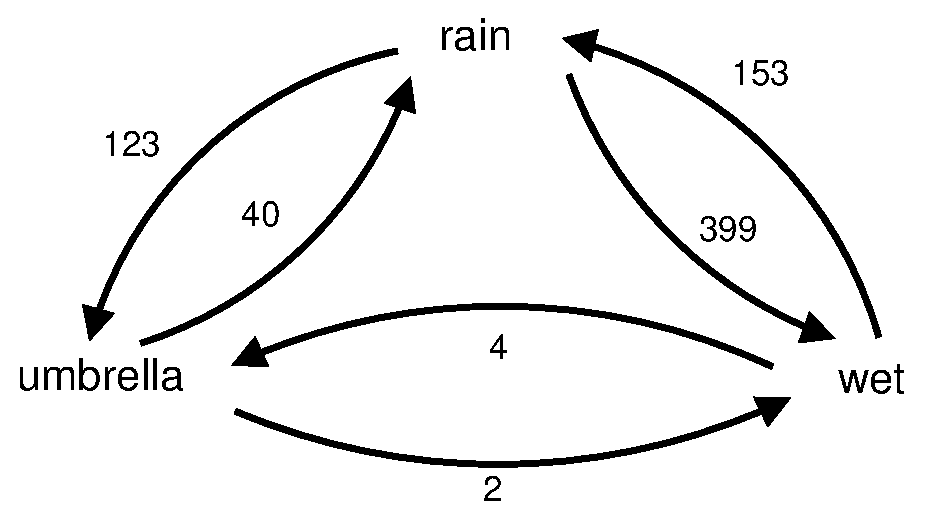
\epsfig{file=causalnet.eps, width=0.6\columnwidth}
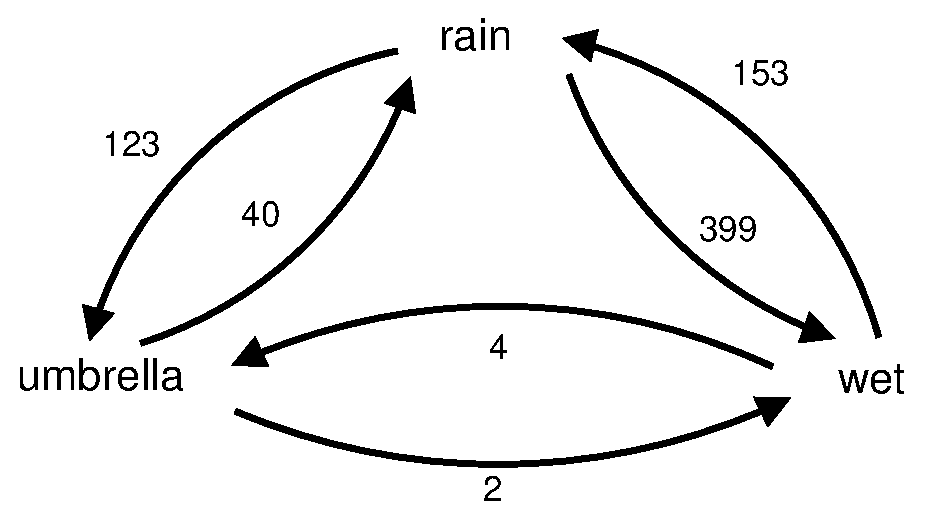
\includegraphics[width=0.7\columnwidth]{causalnet}
\caption{A fragment of causal network}
\label{fig:causalnet}
\end{figure}

\subsection{Causal Strength Computation}
\label{sec:causalstrength}

Text corpus can explicitly as well as implicitly encode causality.
Explicit causality is represented in text
with causal patterns or indicators (e.g., cause, because).
Implicit causality is naturally encoded in discourse without indicators, e.g.,
$A$ appears before $B$ in discourse implies that $A$ is a cause of $B$,
which is more complex and difficult to recognize.
For example,
sentence (1) and (2) explicitly encode causalities using causal patterns,
while sentence (3) encodes the implicit causality
$(\text{loss}_{\text{c}}, \text{sorrow}_{\text{e}})$.

Gordon et al.~\shortcite{gordon2011commonsense} collected implicit causality
from personal story corpus using asymmetric PMI described by Church\shortcite{church1990word},
to achieve the previous best known result on COPA task.
The intuition is that narrations typically describe a series of events
ordered by time. The text that appears earlier tends to be the antecedent
while the text that comes later tends to be the consequent.
Therefore, asymmetric PMI statistics can be used to capture
the implicit causalities encoded in narrative texts such as personal stories.
However, while personal stories might be a good source of implicit causality,
they are hard to come by and limited in scale.
In contrast, using a larger general web corpus improves coverage but
trading accuracy, as web sentences may not follow a narrative pattern.

To leverage the scale and richness of the web text,
we model causality more properly by replacing lexical co-occurrences with
causality co-occurrences extracted by causal cues.
Lexical co-occurrences are weak and implicit causal evidences,
while causality co-occurrences are stronger and more explicit causal
evidences due to the use of causal cues.
Causal cues also help to identify precise cause/effect roles in
strong causal evidences.
Then we propose a new metric to measure causal strength between
two terms with the insight that the connotation of causality
integrates \emph{necessity causality}
with \emph{sufficiency causality}.
Considering a causal pair $(i_c,j_e)$,
necessity causality encoded by $(i_c, j_e)$ represents
that the cause $i$ {\em must} be present in order for
the effect $j$ to take place,
while sufficiency causality encoded by $(i_c, j_e)$ represents
that cause $i$ is all it takes bring about the effect $j$.
For example, the causality $(\text{rainfall}_{\text{c}}, \text{flooding}_{\text{e}})$
in sentence $(2)$  encodes more necessity causality,
since in most situations the effect \textit{flooding} cannot happen
if \textit{rainfall} did not happen as its cause.
Similarly, $(\text{storm}_{\text{c}}, \text{damage}_{\text{e}})$ in
sentence $(1)$ encodes more sufficiency causality.
Intuitively, the stronger the necessity causality is, the larger
the $p(i_c|j_e)$ should be;
the stronger the sufficiency causality is, the larger
the $p(j_e|i_c)$ should be.
We are able to compute such conditional probability because we distinguish
the terms by cause or effect roles. However, the frequent terms are
more likely to be extracted as either causes or effects,
which makes the conditional probability metric bias toward
highly frequent terms.
Therefore, we adopt a more general form (with a penalty factor)
to model the necessity causal strength and
sufficiency causal strength encoded by $(i_c,j_e)$,
as shown in \eqnref{eq:csnec} and \eqnref{eq:cssuf} respectively.

\begin{align}
CS_{nec}(i_c,j_e)  & =  \frac{p(i_c|j_e)}{p^{\alpha}(i_c)} \nonumber \\
                   & = \frac{p(i_c,j_e)}{p^{\alpha}(i_c)p(j_e)}
\label{eq:csnec}
\end{align}
\begin{align}
	CS_{suf}(i_c,j_e) & = \frac{p(j_e|i_c)}{p^{\alpha}{(j_e)}} \nonumber \\
                  & = \frac{p(i_c,j_e)}{p(i_c)p^{\alpha}(j_e)}
,\label{eq:cssuf}
\end{align}
where $\alpha$ is a constant penalty exponent value.
We follow Wettler~\shortcite{Wettler:1993} to set $\alpha$ to be $0.66$,
penalizing high-frequency response terms.
$p(i_c)$, $p(j_e)$ and $p(i_c,j_e)$ are computed as follows:
\begin{equation}
p(i_c) = \frac{\sum_{w\in W}
f (i_c,w_e)}{M}
\end{equation}
\begin{equation}
p(j_e) = \frac{\sum_{w\in W}
f (w_c,j_e)}{M}
\end{equation}
\begin{equation}
p(i_c,j_e) = \frac{f(i_c,j_e)}{N}
\end{equation}
Here, $f(i_c,j_e)$ is frequency of observing the causal pair
$(i_c,j_e)$
from the corpus; $M$ is the total number of evidences, computed as:
$$\sum_{u\in W} \sum_{v\in W} f(u_c,v_e),$$
and $N$ is the size of the corpus;
$W$ is the set of all terms in the causality network.

To show the effectiveness of $CS_{nec}$ and $CS_{suf}$,
we compute the necessity causality and suffiency causality
for causal pairs annotated in SemEval-2010 task 8.\footnote{We further
discuss this corpus in \secref{sec:eval}}
We show the top necessary causal pairs and sufficient causal
pairs ranked by $\frac{CS_{nec}}{CS_{suf}}$ and $\frac{CS_{suf}}{CS_{nec}}$
respectively as shown in \tabref{tab:necsuf}.
% insert the fig:necsuf here
\begin{table}[th]
\caption{Top necessary and sufficient causal pairs}
\label{tab:necsuf}
%\small
\begin{tabular}{l|l}
%\hline intra-sentence cue & inter-sentence cue  \\
Necessary Causal Pairs & Sufficient Causal Pairs \\
\hline \hline
$(\text{man}_c, \text{kidnapping}_e)$ & $(\text{neuroma}_c, \text{pain}_e)$ \\
$(\text{man}_c, \text{jolliness}_e)$ & $(\text{eyestrain}_c, \text{headache}_e)$ \\
$(\text{wind}_c, \text{corkscrew}_e)$ & $(\text{flashlight}_c, \text{light}_e)$ \\
$(\text{rainfall}_c, \text{flooding}_e)$ & $(\text{typhoon}_c, \text{damage}_e)$ \\
$(\text{accident}_c, \text{snarl}_e)$ & $(\text{sunrise}_c, \text{light}_e)$ \\
$(\text{erosion}_c, \text{rill}_e)$ & $(\text{claustrophobia}_c, \text{panic}_e)$ \\
$(\text{crash}_c, \text{gash}_e)$ & $(\text{quake}_c, \text{damage}_e)$\\
$(\text{virus}_c, \text{tonsillitis}_e)$ & $(\text{bacteria}_c, \text{meningitis}_e)$  \\
$(\text{fight}_c, \text{carnage}_e)$ & $(\text{quake}_c, \text{loss}_e)$ \\
$(\text{earthquake}_c, \text{avalanche}_e)$ & $(\text{overproduction}_c, \text{growth}_e)$ \\
\hline
\end{tabular}
\end{table}

Our new causal strength encoded by pair $(i_c,j_e)$ combines
$CS_{nec}(i_c,j_e)$ with $CS_{suf}(i_c,j_e)$,
and is defined in \eqnref{eq:weightedcs}.
\begin{equation}
CS(i_c,j_e) = CS_{nec}(i_c,j_e)^{\lambda} CS_{suf}(i_c,j_e)^{1-\lambda}
%&= \left(\frac{p(i_c|j_e)}{p^{\alpha}(i_c)}\right)^{\lambda}\left(\frac{p(j_e|i_c)}{p^{\alpha}(j_e)}\right)^{1-\lambda}
\label{eq:weightedcs}
\end{equation}
The above metric models both the necessity and sufficiency components
of causality and captures the intuition that
the causal strength should be stronger when both necessity and sufficiency
causality are strong.
Here, $\lambda$ is a parameter, weighing the necessity and sufficiency
causality knowledge that is extracted from text corpus.
A desirable $\lambda$ depends on the characteristics of knowledge
source and extraction methods, as we show in Section~\ref{sec:eval}.

We compute the causal strength between every pair of terms in the
causality network
according to \eqnref{eq:weightedcs}. Where an edge is missing in the network,
we assign a causal strength of zero.

\subsection{Commonsense Causal Reasoning}
\label{sec:reasoning}

To compute whether alternative $a_1$ or $a_2$ is more plausible
with respect to the premise $p$, we need to compare the overall causality
strength $CS_T(p,~a_1)$ and $CS_T(p,~a_2)$, assuming $p$ is asking
for an effect. Here, we compute the causal strength from
text $T_1$ to text $T_2$ as:
\begin{equation}
CS_T(T_1,T_2)=\frac{1}{|T_1|+|T_2|}\sum_{i \in T_1}\sum_{j \in T_2}
CS(i, j)
\label{eq:csall}
\end{equation}

We argue that such simple approach to aggregate causal strength between terms
can effectively model causality between short texts.
The intuition is that each pair of terms drawn from the two texts contribute
to the total causal strength between the two texts. Because $CS(i_c, j_e)$
can be closely related to a probability (with penalty factors),
summing up the causal strength between all pairs is analogous to
computing a pairwise disjunctive probablity.

Furthermore, in our causality model, each term, whether in the cause role
or the effect role, acts as an active agent in contributing causal strength,
either in $CS_{nec}$ or $CS_{suf}$. Each term in the cause role may
cause a number of terms in the effect role and each term in the effect role
maybe caused by a number of terms in the cause role.
Based on this one-to-many relation, we normalize total causality score by
$|T_1|+|T_2|$, which is the total number of agents,
and not $|T_1|\times|T_2|$ presented in previous papers.

One alternative way of constructing the causality network is to extract
causal pairs between phrases instead of terms, since there exists complex
events (e.g., ``catch cold'') that cannot be expressed by a single word.
However, we empirically discovered that such network is less
effective since the frequencies tend to be diluted,
which we report in Section~\ref{sec:eval}, and even though ``catch cold''
is not in our network, we could better capture
phrase causality based on the combined contribution of individual words
``catch'' and ``cold.''

% \input{eval}
\section{Experimental Results}
\label{sec:eval}
In this section, we first give some statistics of
our corpus and the extracted causality network, and evaluate the
quantity and quality of the cue patterns used in the extraction.
We then compared our results on the main COPA task against a number of
existing works using various other data sources and knowledge bases.
Next, we evaluate causality reasoning
on two additional tasks using the data from ConceptNet 4 to
further showcase the power of our framework.
Finally, we demonstrate our network's ability to identify causal directions
using annotated corpus of SemEval-2010 task 8, despite being
agnostic about the context of the input word pairs.
We release the evaluation data used in these experiments
at \url{http://adapt.seiee.sjtu.edu.cn/causal/}.
%\url{http://202.120.38.146/causal}.

\subsection{Data Set and Extraction of Causality Network}
\label{sec:causalnet}
\begin{figure*}[th]
\centering
%\epsfig{file=pattern1.eps, width=1.6\columnwidth}
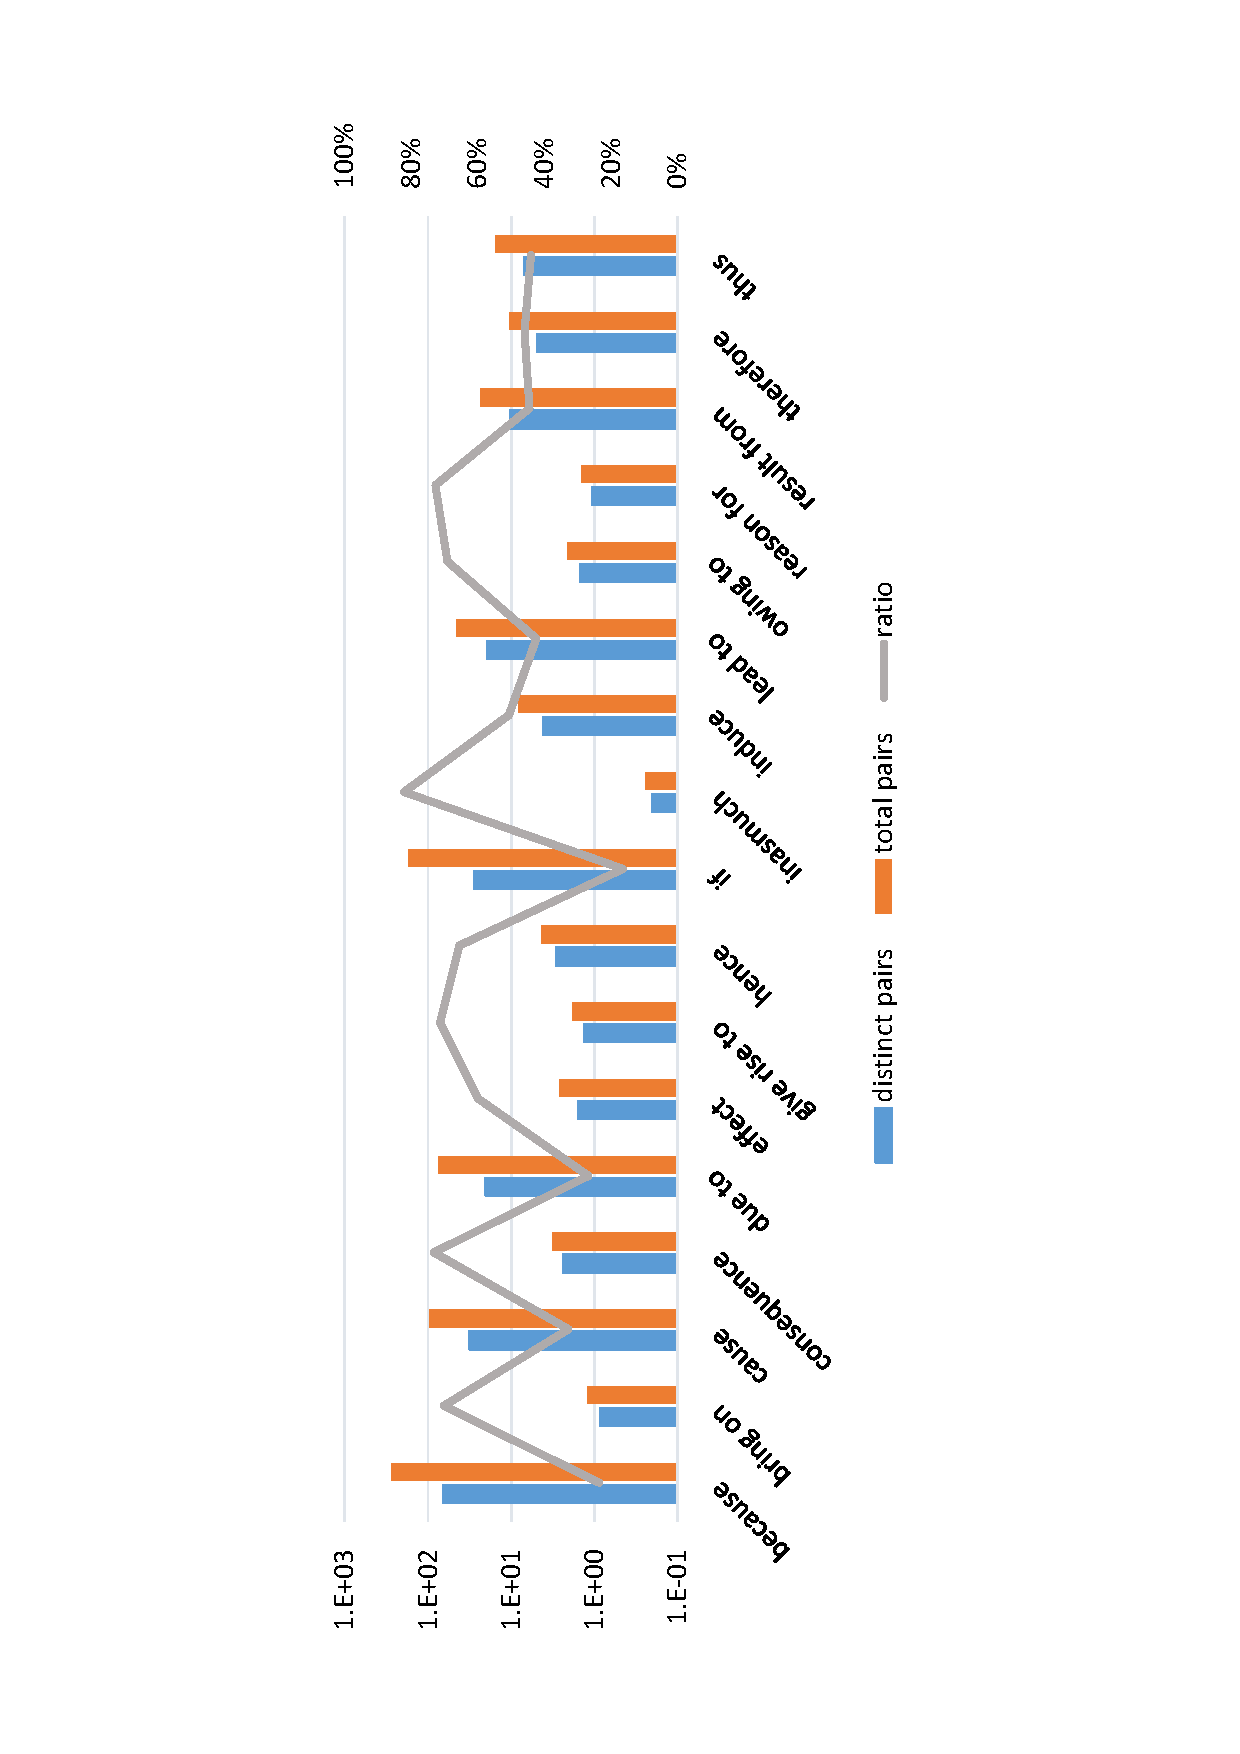
\includegraphics[width=1.6\columnwidth]{pattern1}
\caption{Number of (distinct) pairs extracted by cues}
\label{fig:pattern1}
\end{figure*}
We extracted our term causality network, which we call ``CausalNet''
for convenience in this section, from a large web text corpus (a snapshot of Bing, approximately 10TB), %The snapshot was generated in February, 2013
which contains about 1.6 billion web pages.
We extract 62,675,002 distinct causality evidences (e.g., causal pairs
or edges in CausalNet) from this corpus.
The average frequency of these evidences is 10.54.
The number of unique lemmatized terms (nodes)
in these evidences is 64,436, covering 41.49\% (64,436/155,287) of the
words in WordNet.

As a comparison, we separately extracted an
``event-based'' CausalNet using dependency relations~\cite{chen2014fast}
such as \emph{advmod} and \emph{dobj}.
Only bigram-phrases that match these relations and appear more than
20,000 times in the corpus are considered events; otherwise they are split
into words and paired up as before.
The average frequency on the edges of this event-based CausalNet
is 1.59, much smaller than the orginal CausalNet,
which would make our metric inaccurate due to its sparsity.
Therefore, subquent
experiments are done on the term-based CausalNet.

The 53 causal cues we used can be grouped into 17 sets, each
containing cues of the same meaning or lemma form but with different
tenses. Causal evidences distribution over these pattern sets
is shown in Figure \ref{fig:pattern1}.
The blue bars (left) are the number of distinct
pairs and the orange ones (right) show the total number of pairs.
Inter-sentence cues like ``if'' and ``because'' harvested the
largest number of pairs. But more specialized patterns such as
``reason'' and ``inasmuch'' find more diverse pairs, since the
number of distinct pairs is relatively large compared to the total
pairs extracted.
We show such diversity by the ratio between number of distinct pairs
and number of total pairs
and this ratio is marked by gray line in \figref{fig:pattern1}.

\begin{figure*}[th]
\centering
%\epsfig{file=pattern2.eps, width=1.6\columnwidth}
\includegraphics[width=1.6\columnwidth]{pattern2}
\caption{Number of causal vs. non-causal pairs from ConceptNet covered by cues}
\label{fig:pattern2}
\end{figure*}
To evaluate the quality of the causal cues, we make use of the
manually labeled causal events in
ConceptNet~\cite{liu2004commonsense} as ground truth. ConceptNet 4
contains 74,336 unlemmatized English words, forming
375,135 unique concepts, which are connected by 610,397 relation edges.
Only some of these relations encode causal knowledge,
such as ``Causes'', ``CausesDesire'' and ``HasPrerequisite''.
The total number of such causal relations is 52,778.
Each causal relation also associates with a vote from volunteers.
Those pairs associated with positive votes are annotated as causal pairs
(e.g. (listen to music$_c$, relax$_e$) ),
while associated with negative votes are annotated as false causal pairs
(e.g. (listen to music$_c$, soda can$_e$) ).

Since the pairs from ConceptNet contain
phrases and not just words, we consider a pair ($x$, $y$)
($x$ and $y$ are text spans) to be covered by a
causal cue, if at least one word $u$ in $x$ and another word $v$ in
$y$ form the causal pair $(u_c,v_e)$ which can be extracted word by that cue
from the web corpus.
\figref{fig:pattern2} shows that in general, our cues can
effectively distinguish between positive and negative causal pairs.

\subsection{End-to-end Evaluation on COPA}
COPA task consists of 1000 commonsense causal reasoning questions, divided into
development question set and test question set of 500 each.
The incorrect alternative was purposely set semantically
close to the premise, which makes this task more difficult for
purely associative methods. In this experiment, our parameter $\lambda$
was trained on the development set.
All the reported results are on test set.

To show the usefulness of our causal strength metric, denoted as $CS$,
we compare the end-to-end results on COPA with the
best known PMI statistics on the web corpus.
To solve COPA question with PMI, we pair the terms from
premise and alternative and choose the alternative
with a higher PMI.

We trained our $CS_{\lambda}$ metric
on the development set of COPA
for different data sources (i.e., web corpus and CausalNet).
That means we compute $CS$ based on lexico co-occurrences from web corpus,
while computing $CS$ based on causality co-occurrences from CausalNet.
During the training period,
$CS_{\lambda=0.9}$ and $CS_{\lambda=1.0}$ achieve the same best results
using CausalNet while $CS_{\lambda=0.5}$
performs the best using the web corpus on the development set.
Then we show the performance of these trained $CS$ metrics on test split of COPA.
\tabref{tab:evaluation} shows that
$CS_{\lambda = 0.5}$ on web data
(64.8\%) outperforms PMI with any window sizes.
\tabref{tab:evaluation} also compares $CS_{\lambda=1.0}$ on CausalNet
with several other approaches.
PMI Gutenberg~\cite{roemmele2011choice} uses PMI statistic calculated
from Project Gutenberg (16GB of English-language text).
UTDHLT~\cite{goodwin2012utdhlt} is the
result of SemEval-2012 Task 7 systems. They propose two
approaches. The first one uses PMI over bigrams from LDC Gigaword corpus
(8.4 million documents) as a
feature. The second one treats the task as a classification
problem and combines the features used in the first approach with
some additional features to train an SVM model.
The ConceptNet approach was our own baseline to illustrate the power of
human curated knowledge. Here we fuzzy match
the events or concepts from ConceptNet in COPA sentences, and then compute
the causal strength between two COPA sentences by the scores (e.g.votes)
associated with
causal relations in ConceptNet.
23 out of 500 questions
on COPA test split are matched by ConceptNet,
and 18 of them are correctly answered,
by computing the causality strength between two COPA sentences
from the votes associate with causal relations in ConceptNet.
We just randomly select an answer
for mismatched questions.
The last PMI method~\cite{gordon2011commonsense}, which was also the
state-of-the-art previously (65.4\%), uses a large corpus of
personal stories (37GB of text) with a window of 25.
All competing systems were assessed based
on their accuracy on the 500 questions in the COPA test
split~\cite{gordon2012copa}. Results show that our new metric
$CS_{\lambda=0.9}$$_{/}$$_{1.0}$,
when used together with the automatically harvested CausalNet
achieves significantly better accuracy on the COPA task.

\begin{table}[th]
\small
\centering
\caption{COPA results comparison}
\label{tab:evaluation}
\begin{tabular}{llccc}
\hline
Data Source & Methods & Accuracy(\%) \\
\hline
Web corpus & PMI (W=5) & 61.6\% \\
& PMI (W=10) & 61.0\% \\
& PMI (W=15) & 60.4\% \\
& PMI (W=25) & 61.2\% \\
& {\bf $CS_{\lambda=0.5}$} & {\bf 64.8\%} \\
\hline
Gutenberg & PMI (W=5)  & 58.8\% \\
& PMI (W=25) & 58.6\% \\
\hline
LDC Gigaword & UTDHLT Bigram PMI & 61.8\% \\
 & UTDHLT SVM & 63.4\% \\
\hline
ConceptNet & Fuzzy match & 51.3\% \\
\hline
1-Million Stories & PMI (W=25) & 65.2\% \\
10-Million Stories & PMI (W=25) & {\bf 65.4\%} \\ \hline
CausaNet & {\bf $CS_{\lambda = 1.0}$ } & {\bf 70.2} \%  \\
\hline
\end{tabular}
\end{table}

To further illustrate the effect of web data size on
commonsense causal reasoning, we randomly sample
20\%, 40\%, 60\% and 80\% of our web corpus and thus construct
various CausalNets of increasing sizes. The accuracies of
COPA evaluation using these knowledge bases with $CS_{\lambda=0.9}$
and $CS_{\lambda=1.0}$ are shown in \figref{fig:scale}.
One can observe a general positive correlation between the size of the data
and the ability to reason about commonsense causality. Even at 100\%,
that is the whole of the web corpus available to us, this trend shows
no signs of diminishing, which means, given more data, the results may be
even better. The curves in \figref{fig:scale} also shows a
small bump at 60\% of data.
This is probably due to the randomness in the data distribution (e.g., the
inclusion of certain type of web pages) and doesn't change the overall
scalability of our framework.

\begin{figure}[htb]
\centering
%\epsfig{file=pic2.eps, width=0.9\columnwidth}
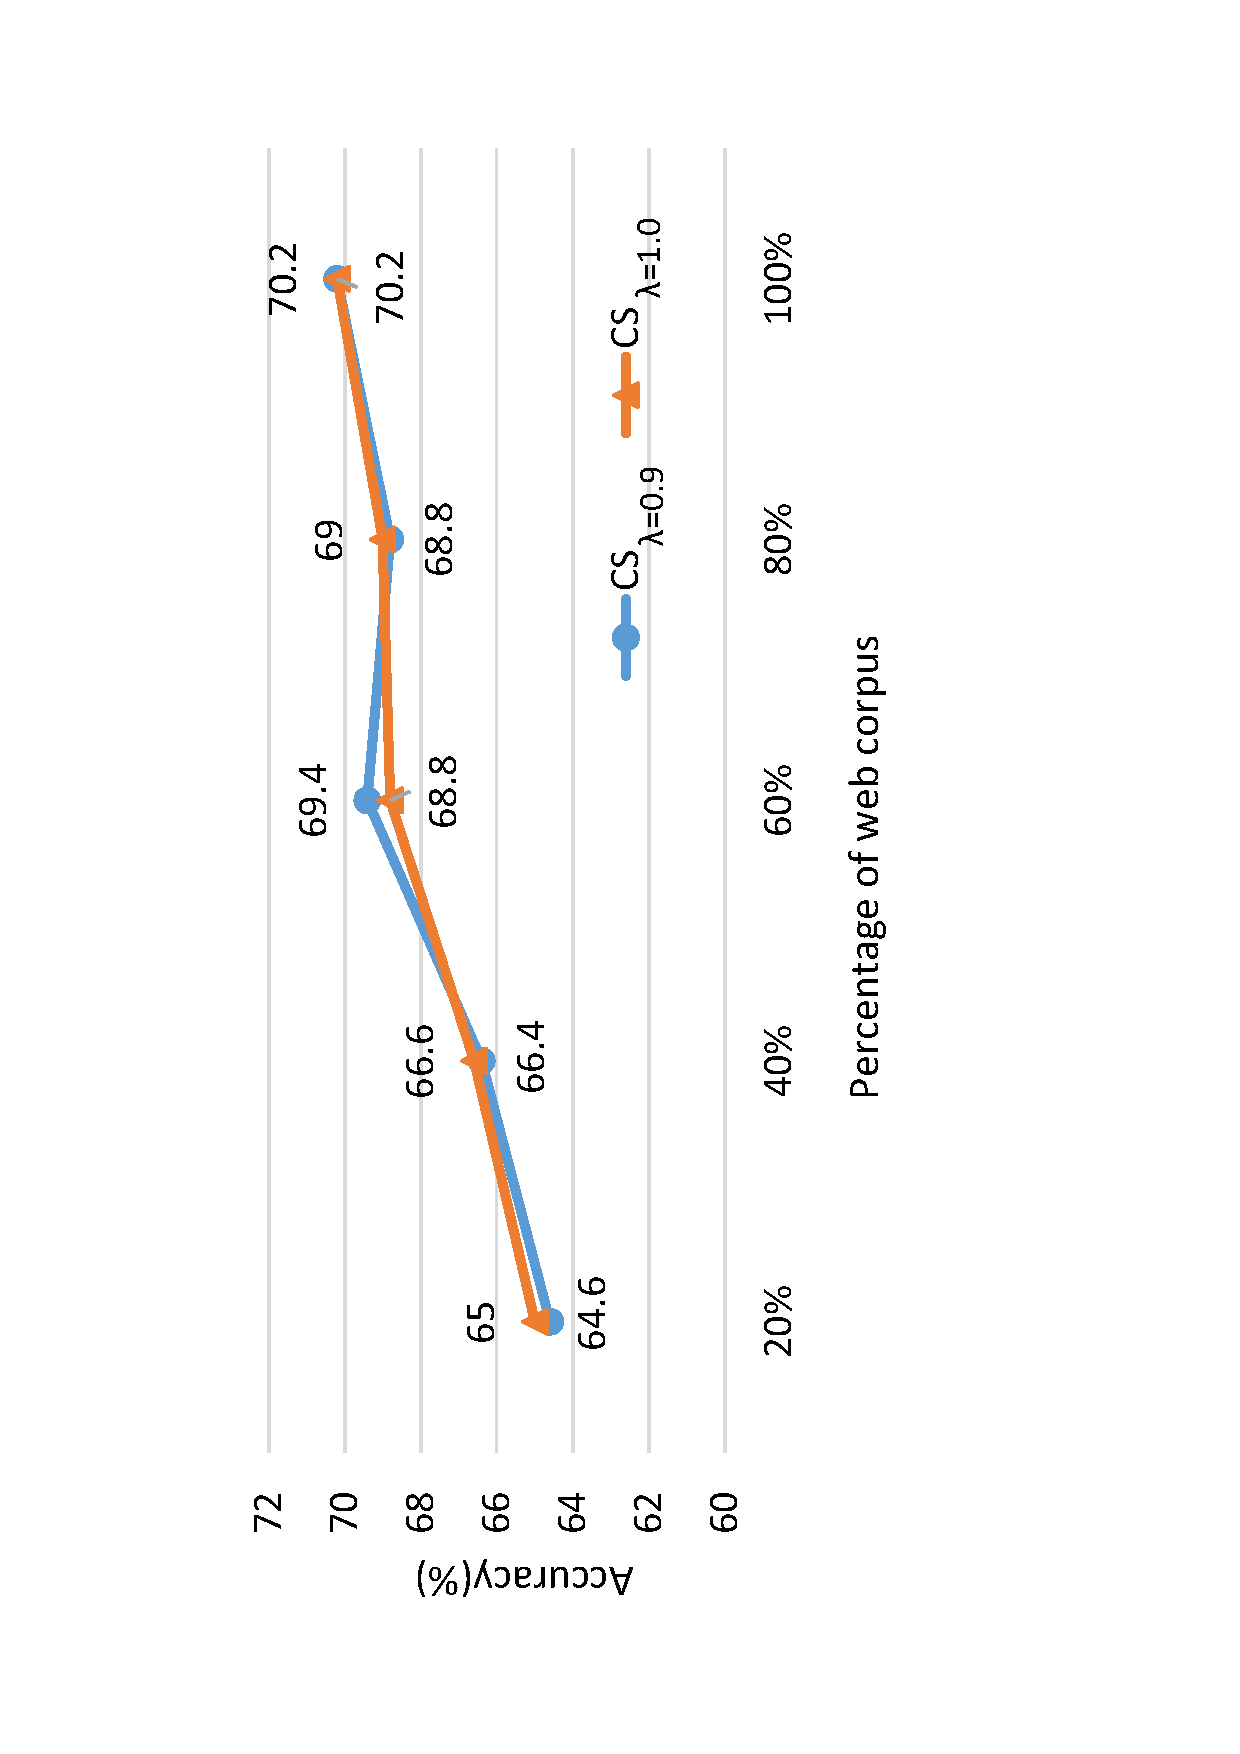
\includegraphics[width=0.8\columnwidth]{scale}
\caption{COPA evaluation on different scales of CausalNet}
\label{fig:scale}
\end{figure}

To understand the effect of $\lambda$ in our metric on
causal reasoning, we conduct more experiments on COPA using different values
of $\lambda$, and on both web corpus and CausalNet. As baselines,
we also include the results using conditional probabilities in
dual directions, $p(i_c | j_e)$ and $p(j_e | i_c)$. The results
are shown in \tabref{tab:varcs}.
Generally, conditional probability underperforms in this task for
both data sources. When computing causal strength using implicit
causality evidences,
the web data is largely unbiased and hence
the causality evidences are observed with roughly
equal sufficiency and necessity causality. Therefore $\lambda=0.5$ gives the best result.
However, when computing $CS$ from CausalNet which is biased
by the explicit causality patterns, a different $\lambda$ is expected.
Because people rarely state ``\textit{A causes B}'' in text explicitly,
when \textit{A} apparently implies \textit{B},
sufficiency causality is seldom observed from CausalNet,
hence a larger $\lambda$ value gives better results.

\begin{table}[th]
\small
\centering
\caption{COPA results for different CS variants}
\label{tab:varcs}
\begin{tabular}{llc}
\hline
Data Source & Methods & Accuracy(\%) \\
\hline
Web corpus & $p(j_e | i_c)$ & 58.2\%\\
 & $p(i_c | j_e)$ & 62.8\% \\
 & $CS_{\lambda=0.5}$ & {\bf 64.8\%} \\
 & $CS_{\lambda=0.7}$ & 63.4\% \\
 & $CS_{\lambda=0.9}$ & 63.0\% \\
 & $CS_{\lambda=1.0}$ & 63.0\% \\
 \hline
CausalNet & $p(j_e | i_c)$ & 56.2\% \\
 & $p(i_c | j_e)$ & 60.2\% \\
 & $CS_{\lambda=0.5}$ & 68.8\% \\
 & $CS_{\lambda=0.7}$ & 69.4\% \\
 & $CS_{\lambda=0.9}$ & {\bf 70.2\%} \\
 & $CS_{\lambda=1.0} $ & {\bf 70.2\%} \\
\hline
\end{tabular}
\end{table}

\subsection{Causality Detection}

Causality detection, or identifying the causal relation in text is
an important task for many applications, such as event prediction,
risk analysis, or decision making support~\cite{mirza2014extracting}.
To show the effectiveness of our work in this aspect,
we investigate the following two research questions on
CausalNet, using data from ConceptNet4.
\begin{itemize}
\item {\bf RQ1:}
For arbitrary event pair manually labeled as \emph{causal} (positive data)
or \emph{non-causal} (negative data), we investigate whether our
proposed causality strength score clearly separates the two.
\item {\bf RQ2:} Inspired by COPA, we select causal and non-causal pairs
sharing the same premise from ConceptNet and form two-choice
questions, to evaluate the ability of CausalNet in selecting the
correct choice.
\end{itemize}

For {\bf RQ1,}
we use the same 200 causal and non-causal event pairs from
\figref{fig:pattern2} as positive and negative data.
\figref{fig:conceptApp1}
%\figref{fig:rq1-0.9} and \figref{fig:rq1-1.0}
shows the causality score $CS_{\lambda=0.9}$ and $CS_{\lambda=1.0}$ ($y$-axis)
of 100 positive
and negative pairs indexed randomly ($x$-axis).
We can observe that scores
of positive and negative pairs are accurately distinguished by a
linear function, %$y=10^{0}$
$y=0.7$, indicated by the gray line.
Consequently, existing systems for causality identification and detection
can incorporate our work to improve their accuracy.

\begin{figure*}[ht!]
\centering
\begin{subfigure}[t]{0.9\columnwidth}
\centering
%\epsfig{file=rq1-09.eps, width=0.9\columnwidth}
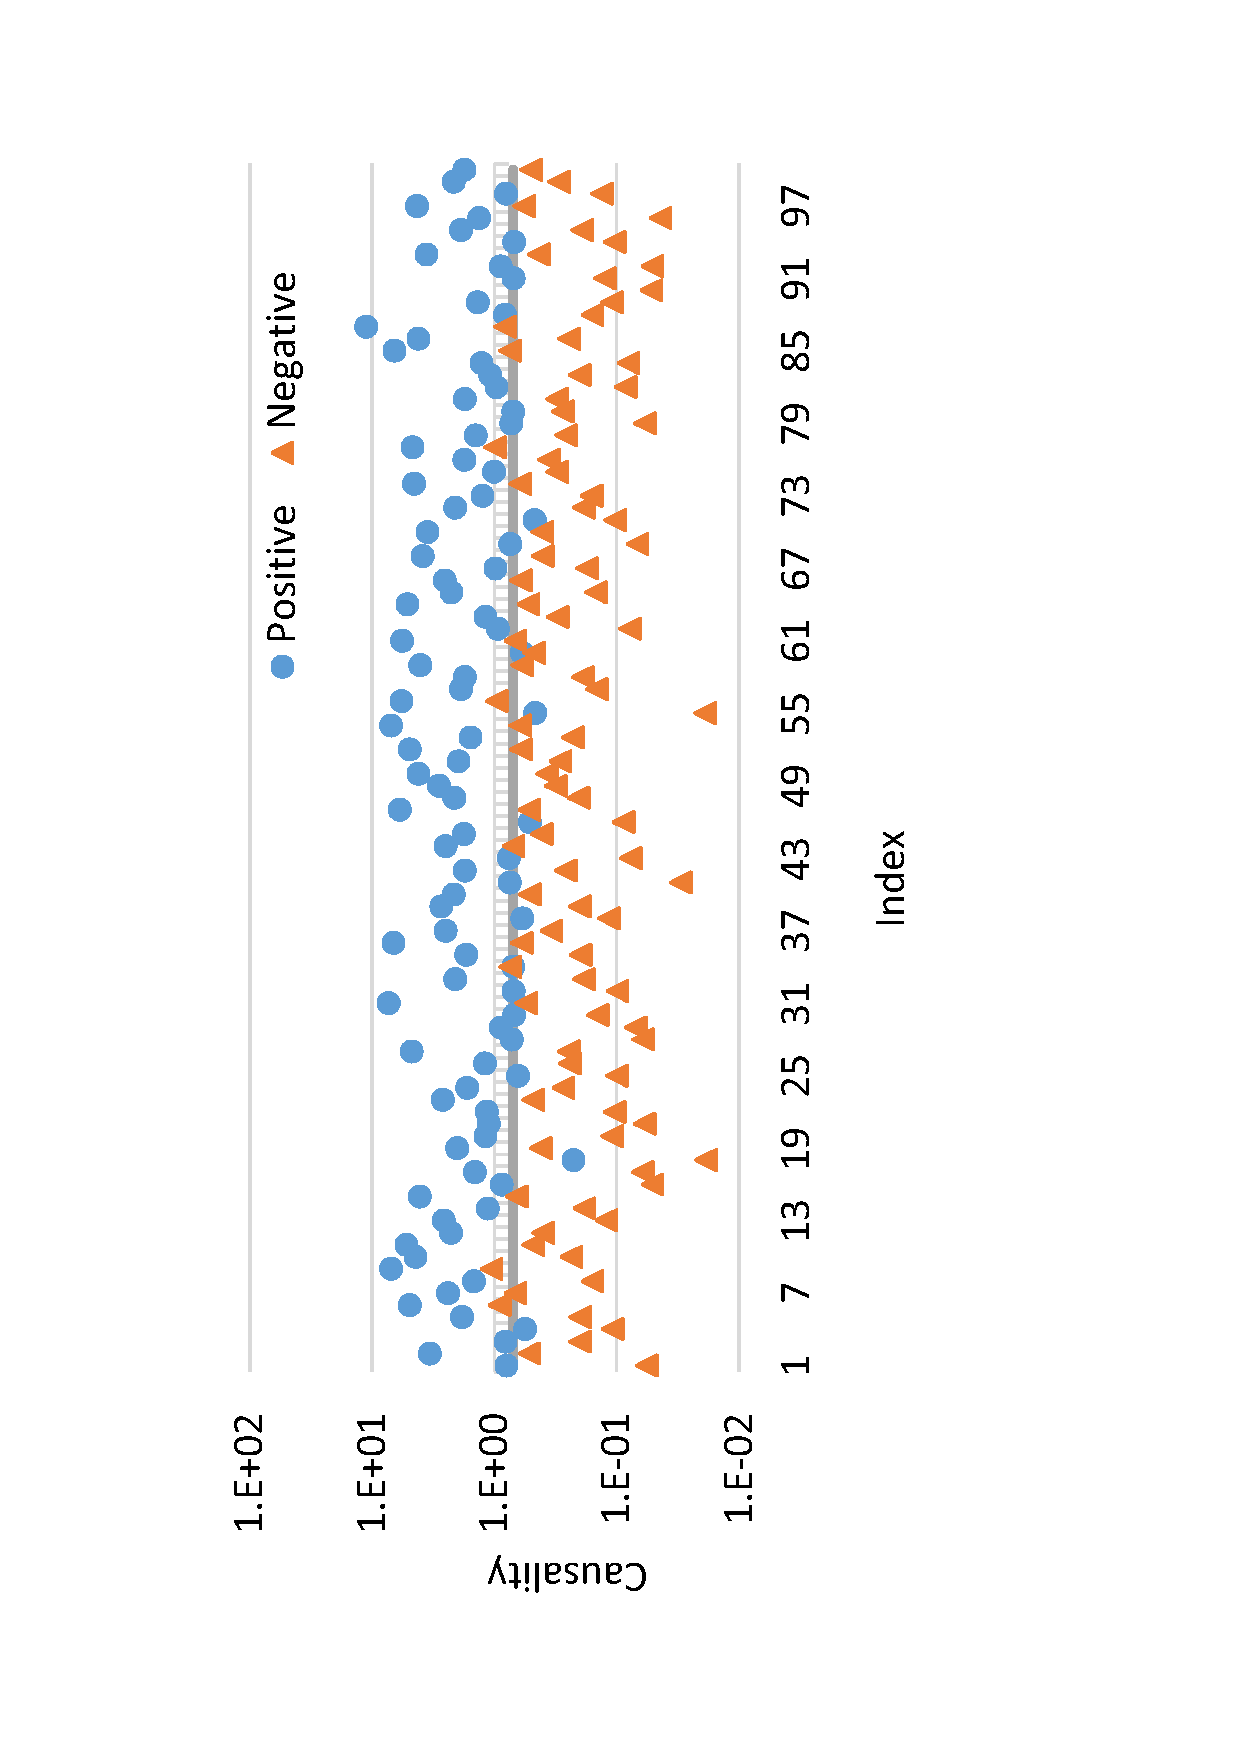
\includegraphics[width=0.9\columnwidth]{rq1-a}
\caption{$CS_{\lambda=0.9}$}
\end{subfigure}
\begin{subfigure}[t]{0.9\columnwidth}
\centering
%\epsfig{file=rq1-10.eps, width=0.9\columnwidth}
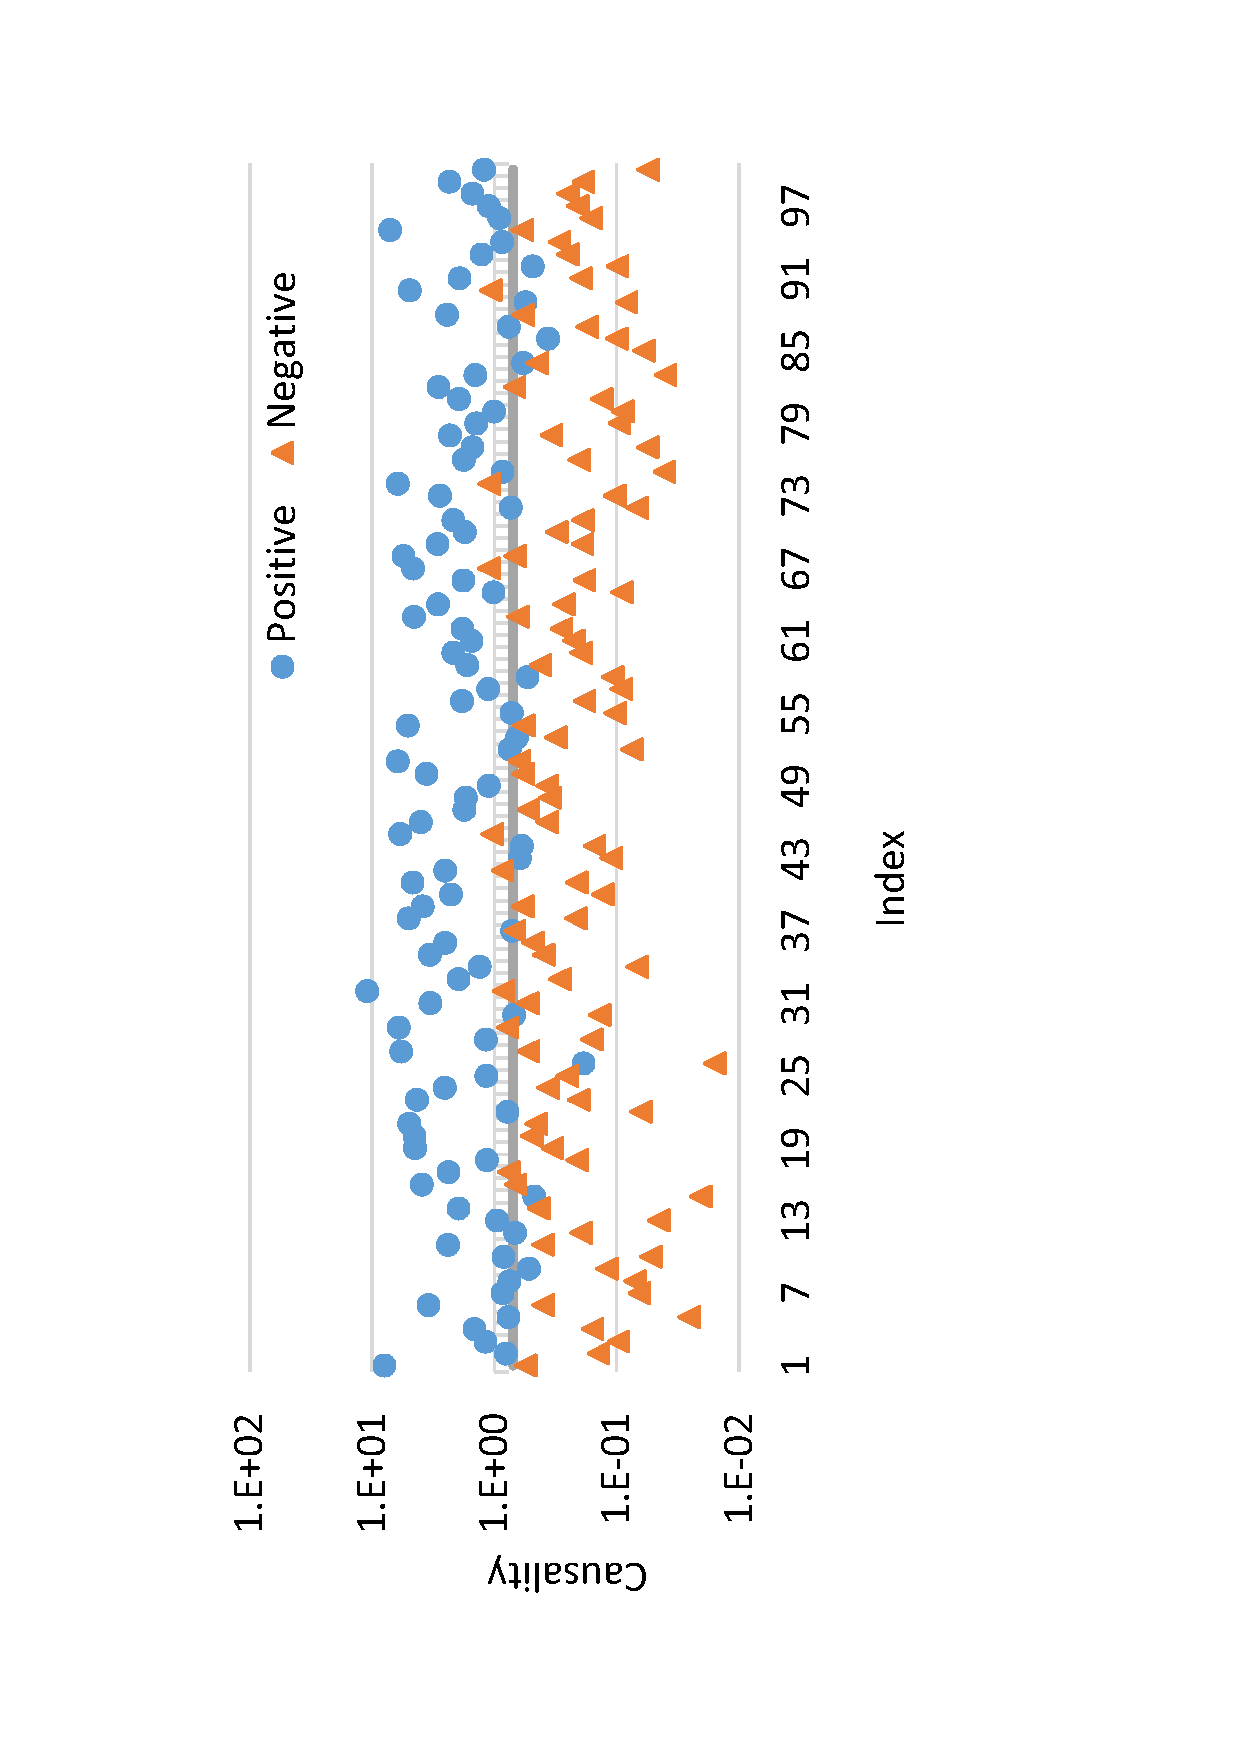
\includegraphics[width=0.9\columnwidth]{rq1-b}
\caption{$CS_{\lambda=1.0}$}
\end{subfigure}
\caption{Distinguishing causality on ConceptNet}
\label{fig:conceptApp1}
\end{figure*}

For {\bf RQ2,}
due to sparsity of pairs sharing the same premise,
we follow \emph{pseudo-disambiguation task} in~\cite{Erk}.
In particular, we use \emph{Causes} relationship $(i,j)$ with
positive votes, such that $i$ is the shared premise and $j$ is a
positive alternative. We then generate a negative alternative
$j'$ without \emph{Causes} relationship with $i$ in randomly selecting.
Since ConceptNet does not exhaustively
label all possible causal relationships, randomly selected $j'$ can
be actually causal, i.e., \emph{false negatives} may exist. In such
situation, we removed the question involving such false negatives,
and consequently obtained a dataset of 412 questions in which 259
look for an effect while 153 look for a cause. \tabref{tab:rq2}
shows that the results of different $CS_\lambda$
using CausalNet.

\begin{table}[th]
%\small
\centering
\caption{Result of ConceptNet RQ2}
\begin{tabular}{cc}
\hline
Methods & Accuracy(\%) \\
\hline
$CS_{\lambda=0.5}$ & 78.4\%  \\
$CS_{\lambda=0.9}$ & 78.6\%  \\
$CS_{\lambda=1.0}$ & 78.6\%  \\
\hline
\end{tabular}
\label{tab:rq2}
\end{table}

\subsection{Direction of Causality}
\begin{table*}[bht]
\centering
\caption{Random samples of annotated causal pairs from SemEval-2010 task 8}
\label{tab:sample}
%\footnotesize
\small
\begin{tabular}{| l c | l c |}
\hline \multicolumn{2}{|c|}{Pairs with match in CausalNet} &
\multicolumn{2}{c|}{Pairs without match in CausalNet}\\
\hline
\multicolumn{1}{|c}{Causal Pair} & \multicolumn{1}{c|}{Commonsense} & \multicolumn{1}{|c}{Causal Pair} & \multicolumn{1}{c|}{Commonsense} \\
\hline
$(\text{vaccine}_c, \text{fever}_e)$ & Yes & $(\text{drink}_c, \text{suffering}_e)$ & Yes\\
$(\text{tension}_c, \text{headache}_e)$ & Yes  & $(\text{malfunction}_c, \text{inflammation}_e)$ & No \\
$(\text{passage}_c, \text{noise}_e)$ & Yes & $(\text{growth}_c, \text{inflammation}_e)$ & No\\
$(\text{injury}_c, \text{discomfort}_e)$ & Yes & $(\text{pie}_c, \text{poison}_e)$ & No \\
$(\text{ash}_c, \text{drama}_e)$ & No & $(\text{city}_c, \text{anger}_e)$ & No \\
$(\text{accident}_c, \text{pain}_e)$ & Yes & $(\text{infection}_c, \text{acne}_e)$ & Yes \\
$(\text{mess}_c, \text{crisis}_e)$ & Yes & $(\text{institution}_c, \text{fraud}_e)$ & No \\
$(\text{pinworm}_c, \text{infestation}_e)$ & Yes & $(\text{dog}_c, \text{joy}_e)$ & No \\
$(\text{parasite}_c, \text{toxoplasmosis}_e)$ & Yes & $(\text{fear}_c, \text{attack}_e)$ & No \\
$(\text{disability}_c, \text{benefit}_e)$ & Yes & $(\text{bacteria}_c, \text{acne}_e)$ & Yes \\
$(\text{elimination}_c, \text{riot}_e)$ & Yes & $(\text{fireplace}_c, \text{warmth}_e)$ & Yes \\
$(\text{generator}_c, \text{signal}_e)$ & Yes & $(\text{tax}_c, \text{fluctuation}_e)$ & No \\
$(\text{drug}_c, \text{unconsciousness}_e)$ & Yes & $(\text{bacteria}_c, \text{breakout}_e)$ & Yes \\
$(\text{zinc}_c, \text{growth}_e)$ & Yes & $(\text{injury}_c, \text{operation}_e)$ & Yes \\
$(\text{reaction}_c, \text{inversion}_e)$ & Yes & $(\text{pregnancy}_c, \text{nausea}_e)$ & Yes \\
$(\text{movement}_c, \text{earthquake}_e)$ & Yes & $(\text{attack}_c, \text{shock}_e)$ & Yes \\
$(\text{virus}_c, \text{disease}_e)$ & Yes & $(\text{lack}_c, \text{reliance}_e)$ & No \\
$(\text{drum}_c, \text{sound}_e)$ & Yes & $(\text{tree}_c, \text{smell}_e)$ & No \\
$(\text{vaccine}_c, \text{outbreak}_e)$ & Yes & $(\text{ointment}_c, \text{discomfort}_e)$ & No \\
$(\text{press}_c, \text{reaction}_e)$ & Yes & $(\text{ginseng}_c, \text{taste}_e)$ & No \\

\hline
\end{tabular}
\end{table*}

Given a pair of terms $i$ and $j$ that are causally related,
CausalNet can generally tell whether the causality is encoded by $(i_c,j_e)$
or by $(j_c,i_e)$ in common sense, without the context of
$i$ and $j$. In other words, as we will show next, CausalNet
provides a reasonable prior knowledge of causality direction.
We use the annotated corpus of SemEval-2010 Task 8 to evaluate this.
There are 920 pairs of terms annotated as Cause-Effect relationship in
SemEval-2010 Task 8 training corpus. CausalNet covered 894 out of
920 pairs (97.2\%).
Each Cause-Effect pair in the SemEval data set is annotated as follows:
\begin{itemize}
  \item[] Sentence:\\
  {\em I too, get a $\langle e1\rangle$ \textbf{headache}$\langle/e1\rangle$
  from $\langle e2\rangle$ \textbf{wine}$\langle/e2\rangle$, and was always told that it was the sulfites.}
  \item[] Relation: \\ \emph{Cause-Effect($e2$,$e1$)}
\end{itemize}
In the above example, $e1$ represents the term ``headache'', and
$e2$ represents ``wine''. The relation Cause-Effect($e2$,$e1$)
indicates that the causality encoded in this sentence is
$(\text{wine}_c,\text{headache}_e)$,
but not
$(\text{headache}_c,\text{wine}_e)$.
We can obtain this useful
insight by the prior knowledge from CausalNet.
We simply compare the causal strength of
$(i_c,j_e)$ with that of $(j_c,i_e)$ provided by
CausalNet. If $CS(i_c,j_e) > CS(j_c,i_e)$($\lambda=0.5$), we
conclude that the causality is encoded by $(i_c,j_e)$,
otherwise the causality is encoded by $(j_c,i_e)$.

The agreement between CausalNet and annotated ground truth in SemEval-2010
Task 8 is 80.1\%, i.e., 716 out of 894 pairs from SemEval find
a matching pair in the same causal direction from CausalNet.
\tabref{tab:sample} shows 20 random samples of annotated causal pairs
from SemEval-2010 Task 8 corpus. 10 of those are matched by
CausalNet and the rest are not. Three human judges were employed to
mark whether these pairs follow common sense or not. A pair
is considered common sense if it is thought so by at least 2 judges.
We can see that all but one pairs in the left column are common sense,
while most of those pairs in the right column are not common sense.
This means, where CausalNet predicts correctly, it is really due to the power
of commonsense knowledge. On the other hand, CausalNet makes mistakes primarily
due to the lack of context in small amount of cases, and not because the
knowledge enclosed is wrong.

% \input{related}
\section{Related Work}
\label{sec:related}

We start by discussing previous work that extracts causal relation term
pairs from open domain text. Then we present various past attempts to
solve the causality reasoning problem.
\cut{We start by discussing previous work that extracts causal relation term pairs
from open domain text.
Then we present various past attempts
to solve the commonsense causal reasoning problem.
}

\subsection{Causal Relation Extraction}
Causal relation recognition and extraction
can be seen as a pre-processing step of causal reasoning.
It naturally boils down to a binary classification problem of
causal/non-causal relations. Existing approaches focus on developing
hand-coded patterns and linguistic features and learning the
classifier to recognize and extract causal relation for their
systems.
Moreover, previous work are specific with
the type of causal pairs and extracted either
noun-noun, verb-verb or verb-noun causation.
Girju et al. \cite{girju2003automatic} were the first to work on
causal relation discovery
between nominals. They semi-automatically extracted causal cues, but only
extracted noun category features for the head noun. Chang et al.
\cite{ChangC04} developed an unsupervised method and
utilized lexical pairs and cues contained in noun phrases as
features to identify causality between them. Both of them ignored
how the text spans surrounding the causal cue
affects the semantics.  Our causal relation extraction
step, instead,  benefits from these contexts and
constructs a much larger and more powerful causal network.
Blanco et al. \cite{blanco2008causal} used
different patterns to detect the causation in long sentences that
contain clauses.
Kozareva~\cite{kozareva2012cause} collected causality relations
between nominals using a bootstrapping method.

Do et al. \cite{do2011minimally} introduced a form of association
metric into causal relation extraction. They mainly focus on
detecting causality between verbs and also worked with verb-noun
causality in which nouns are drawn from a small predefined list.
They used discourse connectives and similarity distribution to
identify event causality between predicate, not noun phrases, but
achieved a F1-score around 0.47. Riaz et al.
\cite{riaz2014recognizing} focus on noun-verb causality detection
and extraction.

None of the previous work except for Do's provides a
causality metric, hence cannot be extended to commonsense causal
reasoning task. Do's work is also of limited help because it only
measures causality strength between verbs.
And most recently, Hashimoto~\cite{hashimoto2015generating} propose
methods to generate reasonable event causalities,
though limited in scale on the event space.  In contrast, CausalNet is
constructed out of all types of words in web corpus, and as a result
the framework on top of it can model the causal strength between
arbitrary text units.
\cut{
Much of the work ignored how the text spans surrounding the causal cue
affects the semantics. Our causal relation extraction
step, instead,  benefits from these contexts and
constructs a much larger and more powerful causal network.
Moreover, previous work
extracted specific types of causal pair, of either noun-noun, verb-verb or verb-noun
\cite{do2011minimally,riaz2014recognizing}
causality. None of the previous work except for
Do's~\shortcite{do2011minimally}
provides a numerical metric to measure causal strength,
hence cannot be extended to causal reasoning between short texts.
Do's work is also of limited help because it only
measures causal strength between verbs.
Recently, researchers \cite{hashimoto2015generating} also propose methods to
generate reasonable event causalities, though limited in scale.
Our CausalNet contains causal strength between arbitrary texts,
by using general web corpus and
extracting nouns, verbs, adjectives and
adverbs.}

\subsection{Commonsense Causal Reasoning}
The causal knowledge which encodes the causal implications of
actions and events is useful in many applications.
Commonsense causal reasoning is thus a
grand challenge in artificial intelligence. Earlier attempts on the
problem were largely linguistic, for example, developing formal
theories to capture temporal or logical properties in causal
entailment \cite{LascaridesAO92,lascarides:asher:1993a}, but
they do not scale to %board-ranging
comprehensive, open domain reasoning problems.

The NLP community has explored knowledge based approaches
that leverage structural representations of the general world knowledge.
Much of the knowledge is hand-coded~\cite{lenat1995cyc}
or crowd-sourced, such as the OMCS project by MIT~\cite{singh2002open}.
Some relations such as ``causes'' and
``causesDesire'' in the ConceptNet \cite{liu2004commonsense},
which is a sub-project under OMCS, can be used to identify causal
discourse in COPA task.
However, such human curated knowledge
has limited size and comes with no or unreliable causal strength
scores (e.g., the votes in ConceptNet).
Recently, several automatic, data-driven methods have
been attempted to acquire commonsense
knowledge\cite{schubert2002can,gordon2010learning,gordon2010mining,akbikweltmodell}.
These approaches focused on the acquisition of general
worldly knowledge expressed as factoids, and not causality knowledge
per se. Hence their coverage of causality knowledge is also very limited.

More successful efforts arise from data-driven approaches
using correlational statistics \cite{gordon2012copa} such as pointwise mutual
information (PMI) between unigrams (words) or bigrams from large
text corpora \cite{Mihalcea2006:CKM}. Corpora attempted include LDC
gigaword news corpus \cite{goodwin2012utdhlt}, Gutenberg e-books
\cite{roemmele2011choice}, personal stories from Weblogs
\cite{gordon2011commonsense} and Wikipedia text
\cite{jabeen2014exploiting}.
This paper follows a similar direction, but instead proposed to extract
causal signals from a more general, much larger web text corpus.
CausalNet can be seen as a large graph-based representation of general
causality knowledge and can provide the relatively reasonable computation of
causal strength between terms.

% \input{conclusion}
\section{Conclusion}
\label{sec:conclude}
This paper proposes a novel framework of
deducing causality by automatically harvesting a
causality network (CausalNet) of causal-effect terms (or causality evidences)
from a large web corpus.
CausalNet is the first (to the best of our
knowledge) automatically constructed graph-based
representation of a causality knowledge base.
This data-driven approach enables
a high coverage including long-tailed causality
relations.
We then propose a novel metric leveraging both sufficiency and
necessary causality evidences
to model the causality strength
between terms.
These metrics between terms can be aggregated for
determining causality
between short texts (e.g., phrases and sentences).
Our evaluation results validate our proposed framework, which outperforms
the previous best approach for solving the competitive SEMEVAL task
known as COPA.

\section*{Acknowledgement}
This work was partially supported by 2014 NSFC-NRF joint research scheme
``Multi-lingual, Cross-cultural Semantic Association Network'', international cooperation program managed by NRF of Korea
(2014K2A2A2000519),  and
NSFC grant No. 61373031.

\bibliographystyle{aaai}
\bibliography{causal}

\end{document}
